\documentclass[12pt]{article}

% Do not forget to crop the pdf: pdfcrop document.pdf document.pdf

% Packages used in the document
\usepackage[margin=1in]{geometry}
\usepackage[utf8]{inputenc}

% Bibliography
\usepackage[backend=biber, style=numeric, sorting=none]{biblatex} 

% Graphics
\usepackage{graphicx}
\usepackage{float}
\usepackage{caption}
\usepackage{subcaption}

% Table formatting
\usepackage{array}
\usepackage{longtable}
\usepackage{pdflscape}
\usepackage{multirow}

% Hyperlinks
\usepackage[hidelinks]{hyperref}

% Special symbols
\usepackage{amssymb}

% Custom commands
\newcommand{\checkedbox}{\item[$\boxtimes$]}
\newcommand{\uncheckedbox}{\item[$\square$]}
\newcommand{\halfcheckedbox}{\item[$\boxdot$]}

% Glossaries
\usepackage[nopostdot,nonumberlist,acronym,toc,section]{glossaries}

% Captions
\captionsetup{justification=centering, font=normalsize}

% Text formatting
\usepackage[normalem]{ulem}

% Title formatting
\usepackage{titling}

% Handling pdf
\usepackage{pdfpages}

\newacronym{ir}{IR}{Infrared}
\newacronym{vis}{VIS}{Visible}

\makeglossaries

\renewcommand{\contentsname}{Table des matières}

\addbibresource{references.bib}

% Redéfinir \maketitle pour ajuster les espacements
\pretitle{\begin{center}\vspace{-3cm}\LARGE} \posttitle{\par\end{center}\vskip
0.5em} \preauthor{\begin{center}\large \lineskip 0.5em}
\postauthor{\par\end{center}\vskip 0.5em} \predate{\begin{center}\large}
\postdate{\par\end{center}\vspace{-1cm}}

\title{Fusion d'images infrarouge thermique et visible à destination de l'humain}
\author{Aurélien Godet}
\date{1er CSI : 15/07/2024}

% Start of the actual document content
\begin{document}
\maketitle

\printglossary[type=\acronymtype, title=Liste des Acronymes]
\printglossary[type=main,title=Glossaire]

% -------------------------------------------------------------------------------

\addcontentsline{toc}{section}{Bibliographie}
\printbibliography

% -------------------------------------------------------------------------------
\newpage
\section{Introduction}
La fusion d'image infrarouge et visible est un domaine de recherche 
en pleine expansion dans la vision par ordinateur, visant à améliorer 
la perception humaine en combinant les informations issues de différentes 
bandes spectrales. Cette technique est essentielle pour diverses applications, 
telles que la surveillance, la navigation et la conduite autonome, 
ou le diagnostique thermique, où chaque type d'image apporte des informations 
complémentaires. Les images visibles fournissent des détails texturés et 
colorimétriques, tandis que les images infrarouges révèlent des informations 
thermiques, souvent cruciales dans des conditions de faible luminosité ou à 
travers des obstacles tels que la fumée ou le brouillard.

J'ai concentré mon début de travail de thèse à rester à jour avec les progrès dans 
ce domaine en consultant régulièrement la littérature et à développer une solution 
pour réaligner les images visibles et infrarouge du dataset mis à disposition par LYNRED.
Ce genre de thématique a été largement abordé ces dernières années, car les paires multimodales
non alignées sont bien plus difficile à utiliser pour obtenir une fusion net avec des
contours précis et des textures nettes. Un mauvais alignement de deux images peut donner des frontières 
dupliquées et à une perte important d'information par recouvrement de certaines zones.

\begin{figure}[h!]
    \centering
    \begin{subfigure}[b]{0.45\textwidth}
        \centering
        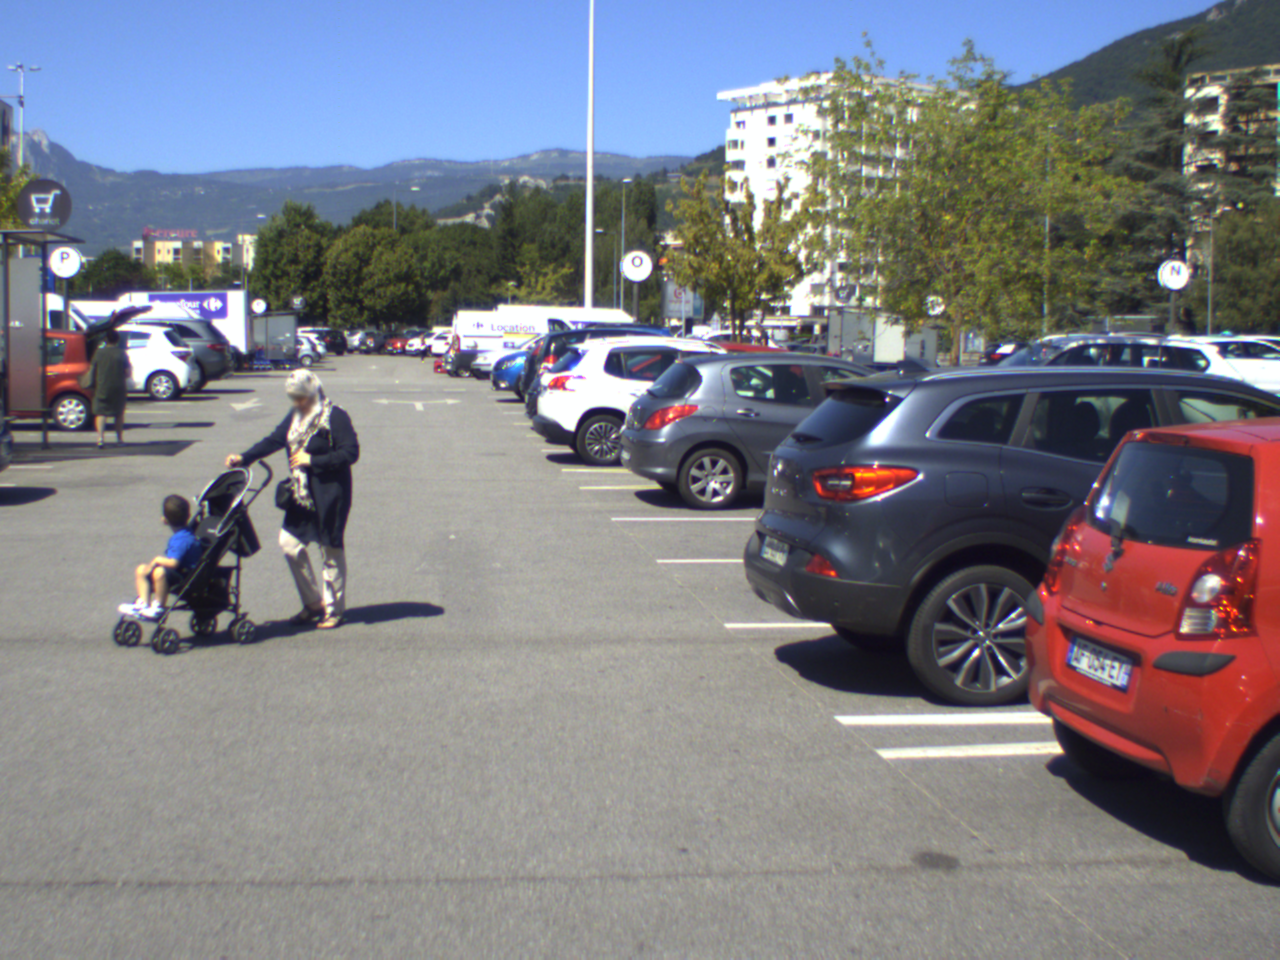
\includegraphics[width=\textwidth]{images/VIS.png}
        \caption{Caméra visible gauche (1280, 960)}
        \label{fig:vis_exemple}
    \end{subfigure}
    \hfill
    \begin{subfigure}[b]{0.45\textwidth}
        \centering
        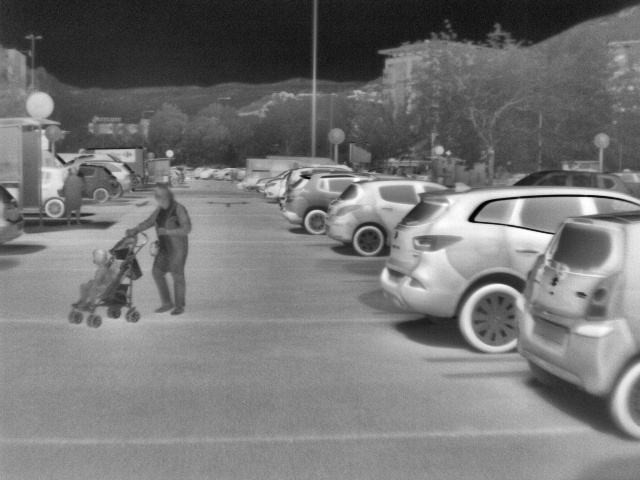
\includegraphics[width=\textwidth]{images/IR.png}
        \caption{Caméra infrarouge gauche (640, 480)}
        \label{fig:ir_exemple}
    \end{subfigure}
    \caption{Paires d'images type non alignées du Dataset LYNRED}
    \label{fig:two_images}
\end{figure}


% -------------------------------------------------------------------------------
\newpage
\addcontentsline{toc}{section}{Récapitulatif de participation aux formations}
% \includepdf[pages=-, scale=0.9, pagecommand={}]{attachés/récapitulatif_formation_adum.pdf}

\end{document}